%% thesis.tex 2022/2/14
%
% Based on sample files of unknown authorship.
%
% The San Francisco State University LaTeX thesis template is
% derived from the UC Berkeley LaTeX thesis template. 
%
% The current maintainer of this work at San Francisco State University is Robert Browder.
%
% A healthy alternative to working directly in LaTeX is to use the thesisdown or bookdown package with R Studio.
% Thesis down provides the opportunity to embed executable code within the narrative flow of your document.
% Thesis down provides both PDF and HTML output.  
%
% This is the main file for this template
%
% This file is where authors may customize title, author, degree semester, degree year, degree, 
% chair, other members, and major.
%
% This file issues the commands to include each part of the document, 
% Pre-formatted parts available - abstract, preface, acknowledgments, introduction, chap1, chap2, 
% and references
% Any part can be omitted by commenting out its "include" command
% Authors may also rearrange the order of contents and add additional chapters using the mark-up examples provided


\documentclass{sfsuthesis}
\usepackage{biblatex}

% Use the graphix package with dvipdfmx when exporting to HTML to preserve figure dimensions for JPG and PNG file types. 
% For this to work you must first create an .xbb file for each file using the following command from the CLI
% ebb -x Picture2.jpg
% \usepackage[dvipdfmx]{graphicx}

% Use the graphix package without dvipdfmx when exporting to PDF
\usepackage{graphicx}
\usepackage{amsmath}
\usepackage{rotating} % provides sidewaystable and sidewaysfigure

% To compile this file from the command line, run "latex thesis", then "biber thesis"
% (or "bibtex thesis", if the output from latex asks for that instead),
% and then "latex thesis" (without the quotes in each case).
%
% Alternatively, use Overleaf, MacTeX, or MikTeX to compile to PDF.
%
% To compile this file to HTML from the command line, run 
%  make4ht -f html5+mjcli thesis.tex "mathjax"
% this step requires Nodes.js, MathJax, and mjcli.js to be installed and working on your machine


% comment out the following two lines for single spacing
\def\dsp{\def\baselinestretch{2.0}\large\normalsize}
\dsp

% comment out the following line to control indentation of the first paragraph of a section
\usepackage{indentfirst}
\usepackage{appendix}

\addtolength{\abovecaptionskip}{\baselineskip}

\newtheorem{theorem}{Sample Text}

\bibliography{references}

\hyphenation{mar-gin-al-ia}
\hyphenation{bra-va-do}

%path to the folder which contains figures
\graphicspath{ {./figures/} }

\begin{document}

% Declarations for Front Matter

\title{Title of Culminating Experience}
\author{First Middle Last Name}
\degreesemester{May}
% Select one of the semesters: December, May, or August.
\degreeyear{20XX}
% Enter the year in which you are submitting your thesis.
\degree{Masters of - Your Degree here -}
%example: Masters of Science
\chair{Name of Committee Chair}
\chairdegree{Ph.D}
\chairrank{Professor}
\cochair{Name of Co-chair}
\cochairdegree{Ph.D}
\cochairrank{Associate Professor}
\memberthree{Name of Member Three}
\memberthreedegree{Ph.D}
\memberthreerank{Associate Professor}
\memberfour{Name of Member Four}
\memberfourdegree{Ph.D}
\memberfourrank{Associate Professor}
\othermembers{Professor Roger Spam \\
  Associate Professor Michael Chex}
% For a co-chair who is subordinate to the \chair listed above
% \cochair{Professor Benedict Francis Pope}
% For two co-chairs of equal standing (do not use \chair with this one)
% \cochairs{Professor Richard Francis Sony}{Professor Benedict Francis Pope}
\numberofmembers{3}

\field{- Your Major: Concentration here - }
% Example: Computer Science: Software Engineering
% Designated Emphasis -- this is optional, and rare
% \emphasis{Colloidal Telemetry}
% This is optional, and rare
% \jointinstitution{University of Western Maryland}
% This is optional (default is Berkeley)
% \campus{Berkeley}


\maketitle
% Delete (or comment out) the \approvalpage line for the final version.
\copyrightpage
\approvalpage


% (This file is included by thesis.tex; you do not latex it by itself.)
\begin{abstract}

% The text of the abstract goes here.  If you need to use a \section
% command you will need to use \section*, \subsection*, etc. so that
% you don't get any numbering.  You probably won't be using any of
% these commands in the abstract anyway.

T-cells are one of the key components of the adaptive immune system. T-cell Receptors (TCR) are a group of protein complexes found on the surface of T-cells. TCRs are responsible for recognizing and binding to certain antigens found on abnormal cells or potentially harmful pathogens. Once the TCRs bind to the pathogens, the T-cells attack these cells and help the body fight infection, cancer, or other diseases. TCR repertoires, which are continually shaped throughout the lifetime of an individual in response to pathogenic exposure, can serve as a fingerprint of an individual’s current immunological profile. The similarity among TCRs sequence directly influences the antigen recognition breadth. Network analysis, which allows interrogation of sequence similarity, thereby adds an important layer of information. Due to the heterogeneous nature of TCR network properties, it is extremely difficult to perform statistical inference or machine learning directly between subjects. In this work, a novel method is proposed to prioritize the network properties that are associated with the outcome of interest, based on features extracted from heterogeneous global/local network properties. Schemes to select the top features associated and to simulate the network properties using the real data are also presented.  Extensive simulation studies and real data analysis were performed to demonstrate the proposed methods. Performance measures including F-1 score, false discovery rate, sensitivity, power, and stability were calculated for each model and are used for model comparison.

\end{abstract}


\begin{frontmatter}

\begin{preface}
\begin{comment} I owe it all to my supervisor Professor Reinhard Furrer for his guidance throughout this project.
His insights and intuition for numerical methods have been most memorable lessons for me.
I would also like to thank Professor Barbara König for not only giving interesting research
questions, but also for giving me such a rich lesson about animal behavior. My thanks also goes
to Dr. Julian Evans for his help with the data set and advice.
This thesis is but a culmination of my master program, and for that, I would also like to thank Dr.
Eva Furrer for all her care in ensuring that we have received the best education and experience. I
would also like to thank Professor Leonhard Held and Dr. Ulrike Held, who taught me practical
biostatistics.
Last but not least, thank you to my family for always believing in me.
Sandar Felicity Lim
November 2019
\end{comment}
\end{preface}

% You can delete the \clearpage lines if you don't want these to start on
% separate pages.


\begin{acknowledgments}
I would like to begin by thanking my supervisor Dr. Tao He, whose invaluable guidance and support helped me through each step of my thesis and taking it to completion. Thank you Dr. Tao He for being patient and always present for my questions. I am grateful to Dr. Li Zhang and her team, from UCSF (University of California San Francisco) for collaborating with us on this work. I would like to extend my deepest gratitude to the committee members, Dr. Mohammad R. Kafai and Dr. Alexandra Piryatinska for their support and valuable feedback.\par

I can never be grateful enough to my friends and family for their unwavering support and encouragement throughout my graduate program. Especially my mother, Mrs. Seema Banerjee, my husband, Dr. Aritra Sengupta, my sister, Nabanita Banerjee and my in-laws. Thank you for being there for me emotionally and intellectually as I worked through my coursework. I would like to dedicate this work to my father, Late Pronab Kumar Banerjee, who taught me to dream big and to never give up on my pursuits.\par

Finally, I would like to thank the mathematics department and the SF Build committee for the Bridge Award and the SF Build Agent of Change scholarships that allowed me to conduct my thesis.\par

This work was supported in part by the National Science Foundation (NSF DMS-2137983) and the National Institute of Health (NIH/NCI R21CA264381 and NIH/NLM R01LM013763-01A1).
\end{acknowledgments}

\tableofcontents
\clearpage
\listoftables
\clearpage
\listoffigures
\clearpage

\end{frontmatter}

% (This file is included by thesis.tex; you do not latex it by itself.)
\chapter{Introduction}

% If you need to use a \section
% command you will need to use \section*, \subsection*, etc. so that
% you don't get any numbering.  You probably won't be using any of
% these commands in the abstract anyway.

T cells are crucial components of the adaptive immune system, mediating anti-tumoral immunity and immune response to infections. They are necessary for effective host-response to a wide range of pathogens. T cells are defined by their T cell receptors (TCRs), which are protein complexes on the T-cell surface. TCRs mount a response to harmful foreign invaders by targeting specific antigens based on nucleotide sequence. TCRs act as the arms of the T cells with memory and can remember harmful pathogens they have seen before, thereby providing a life-long protection which enables a swift response in case of a similar future encounter. Thus, understanding the TCR repertoire could lead to insights regarding immune response pathology while also discovering indicative bio-markers and lead to therapeutic strategies.\par

As the immune repertoire ages, it is shaped based on the environmental exposure of an individual throughout their lifetime. Therefore, performing statistical inferences directly on TCR data between subjects is challenging due to its heterogeneous nature. In fact, there is less than 20\% overlap across repertoire, even for the same subject. However, it is observed that the similarity among TCRs sequence directly influences the antigen recognition breadth. Therefore, interrogation of TCR sequence similarity can add an important layer of information. This can be achieved through network property analysis of TCR repertoire. A clonal network is constructed where each clone is defined as a node, and then based on the sequence distance (Levenshtein distance), an edge is drawn based on a certain similarity condition (e.g., one letter difference in sequence).\par

\section{Background}\label{sec:background}
In this work we analysis the data of 65 patients from the Phase I trial (NCT01693562, 14 September 2012)  of durvalumab, an immune checkpoint inhibitor (ICI) designed to activate exhausted tumor-reactive T cells. Durvalumab consolidation therapy is administered to patients with stage III, non-small cell lung cancer (NSCLC) and their immunophenotypic responses are observed. The patients exhibiting increased TCR repertoire diversity on day 15 attained significantly longer overall survival (OS) than those with decreased diversity. Patients with larger TCR clusters showed improved OS than patients with smaller TCR clusters (\cite{lizhang}Elliot Naidus \textit{et al.}, 2021). It was inferred that early TCR repertoire diversification after durvalumab therapy for NSCLC may be predictive of increased survival. Therefore, drawing quantitative analysis of the TCR repertoire in \lq longer overall survival' and \lq shorter overall survival' cohorts may provide a better understanding of the immune landscape involving T cell response. This information can then be used to develop tools to improve patient stratification, prediction of disease outcome, and patient response to treatments.\par

\section{Motivation and Objective}\label{sec:motiv_objctv}
The immunophenotypic response data captures the TCR repertoire details for the 65 patients. The TCR repertoire data is continually shaping over a patient's lifetime and is also impacted as a response to the immunotherapy administered to the patient, thereby making the data heterogeneous in nature. The network data available for our analysis was extracted by sequencing the TCR repertoire. This network data is shown in the \autoref{fig:nw_prop}. A total of fifteen network properties of the TCR repertoire data are used for this work which are referenced as the TCR network properties collectively. Some of these network properties are global and some are clonal (local) network properties (\cite{tcr_ntw}Miho \textit{et al.}, 2019). Another data set representing the overall survival stats for these 65 patients was also referenced. It was also made available that the patients with overall survival months ($OS\_mon$) $\ge 20.3$ have a higher survival chance than the other patients. For the analysis, the network properties are used as the explanatory variables and the overall survival month ($OS\_mon$) as the response variable. Patients with $OS\_mon$ $\ge 20.3$ are categorized into \lq longer overall survival' group and patients with $OS\_mon<20.3$ are categorized into \lq shorter overall survival' group. The objective here is to investigate the TCR repertoire network properties and develop novel statistical method to prioritize the important network properties that are associated with the clinical outcome of increased overall survival.\par
\begin{figure}[H]
\centering
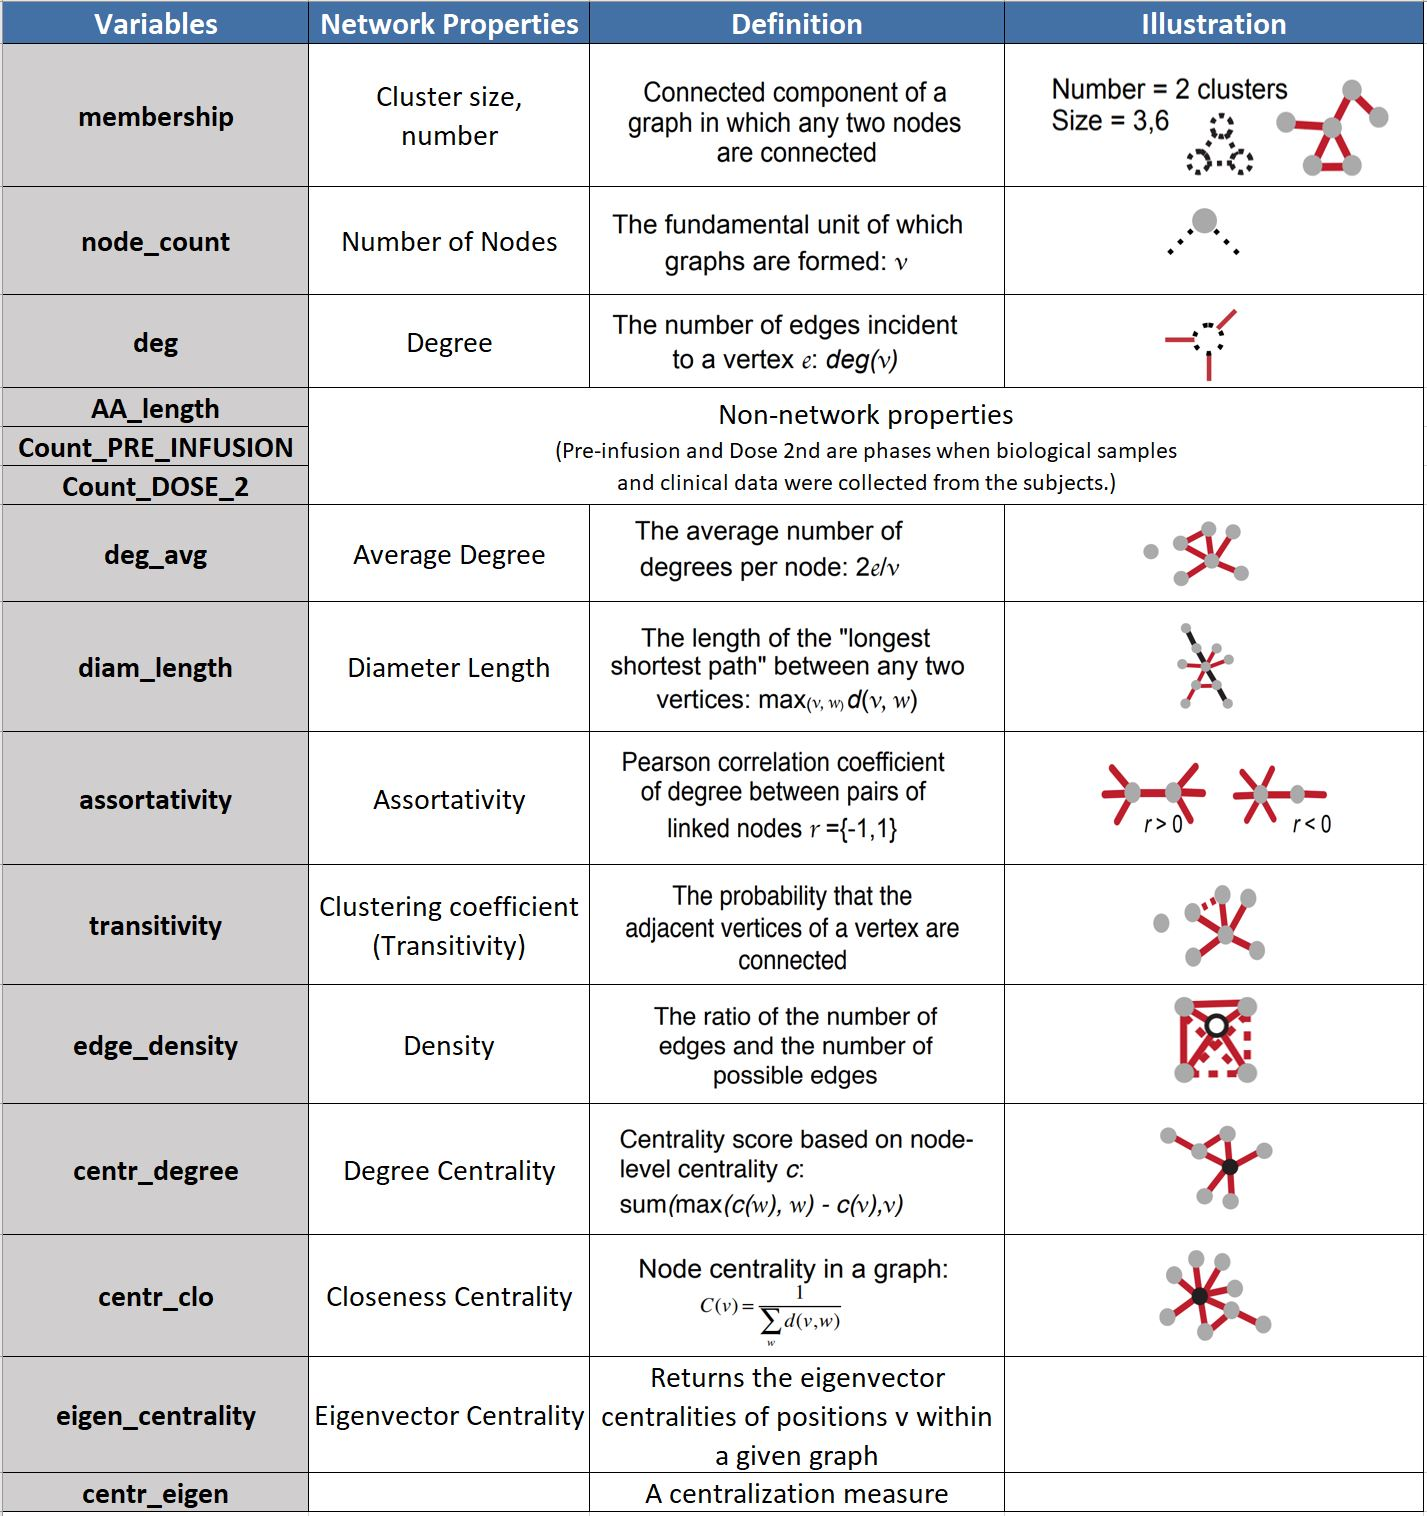
\includegraphics[scale=0.75]{NetworkProperties}
\caption{TCR network properties used for analysis (\cite{tcr_ntw}Miho \textit{et al.}, 2019).}
\label{fig:nw_prop}
\end{figure}

\section{Challenges}\label{sec:challenges}
The response variable, $OS\_mon$, has a definite value for each of the 65 patients. The TCR network data (the explanatory variables) consists of a mix of global and local variables. The global variables are described by a single set of values, while the local variables are vectors of varying lengths. Since the TCR repertoire is constantly adapting to the health and the environmental factors of the patient, the network properties are continually shaping. Given any two patients the TCR repertoire is never the same. Less than 20$\%$ overlap is observed in the TCR repertoires for the same subject. This heterogeneous nature of the TCR repertoire and network properties makes it difficult to perform statistical inference or machine learning directly between subjects. The heterogeneity issue also complicates the data simulation process required to perform the simulation study. Therefore, we require to develop ingenious ways to handle the TCR network data throughout this work and make it suitable to run statistical inferences.\par

\section{Contribution}\label{sec:contribution}
In this paper we proposed a strategy to extract features from the heterogeneous global/local network properties. Reading through the distribution of the network properties using the real data, we collect some summary statistics. These derived summary statistics (referred to as the \lq network features') largely consist of the Minimum, the $1^{st}$ Quartile $(Q_1)$, the Median, the Mean, the $3^{rd}$ Quartile $(Q_3)$ and the Maximum values. This technique is uniformly repeated for all the properties. The network properties are then represented by aggregating these summary statistics (referred to as the \lq feature blocks/groups'). This approach helps to sum up the TCR network properties for each patient and renders the data suitable for making statistical inferences.\par

We then apply variable selection techniques like Lasso (\cite{tibshir}Tibshirani, 1996), Group Lasso (\cite{grouporigin}Yuan and Lin, 2005), and Exclusive Lasso (\cite{exclusv_lasso}Zhou, Jin and Hoi, 2010) to prioritize the T-cell Receptor (TCR) network properties and to select the top network features. The technique of Group Lasso is applied to the feature blocks. This helped with identifying the significant feature blocks. Next, the Lasso and Exclusive Lasso techniques were used to identify the top performing network features. In conjunction with variable selection methods, the cross-validation technique is generally used to render the optimal tuning parameter $\lambda$ those aids in shrinking and selecting the significant variables. Through this work we presented a comparison of how the cross-validation technique performs against a new technique called the permutation-assisted tuning. This new technique uses a permutation copy of the original data set, with the intention of disrupting the structure existing between the response variable and the explanatory variables. This creates a data set with pseudo-variables that has the same dimensions as the original data set. The final data is widened (predictor space is doubled) by augmenting both the original data set (using the true active variables) and the permutation copy (using the pseudo-variables). The modified data is then fed into the variable selection algorithms to identify a tuning parameter $\lambda$ such that the pseudo-variables are never selected. The permutation tuning technique is known to have lower false positives than the cross-validation technique. So far, the permutation assisted tuning has been used only on Lasso models. We add novelty in expanding its application to Group Lasso models and present how this technique can be used to identify the significant feature blocks. During this work we also deduced that the permutation assisted tuning method cannot be applied to Exclusive Lasso models when trying out with decreasing $\lambda$ values. The Exclusive Lasso model bounded by its design selects at least one feature from every existing feature block. Hence, Exclusive Lasso will never converge to find a $\lambda$ value which can differentiate between the true variables and the pseudo-variables when using permutation tuning.\par

We proposed a procedure to simulate the network properties using the real data such that the correlation structure between the predictors is preserved. The network property distributions gave us an insight to some of the correlations that exist among the explanatory variables. Using approximate correlation structures, we first simulated a heterogeneous form of the TCR network data and then aggregated it using the summary statistics technique proposed earlier. The simulated data set gave us the flexibility to compare the model performances and ensured the soundness of the results using various performance measures like --- Sensitivity, False Discovery Rate, F1 score, Power, and Stability.\par

We provide the results of our analysis from the original data set, where we captured the significant network properties (feature blocks) and network features (summary statistics). To validate those results and compare between the different variable selection methods we perform the simulation study. In this section we present an alternative technique than GPUs to perform large-scale network data simulation. Analyzing the network properties, identifying the superficial dependencies and correlations guides us to simulate the network data. The simulated data is then fed into the previously used variable selection models and performance measures like - Sensitivity, False Discovery Rate, F1 score, Power and Stability are computed. We observe that the permutation assisted tuning method, used to derive the tuning parameter, outperforms the cross-validation technique when performing variable selection. We finally present the set of significant network properties and the top network features that contribute to determining increased overall survival months in the patients.\par



\pagestyle{headings}

% (Optional) \part{First Part}

\include{chap1}
\include{chap2}

\printbibliography

\appendix
\addappheadtotoc



\section{Appendix A: List of California State University Campuses}

\begin{itemize}
\item California State University, Bakersfield
\item California State University Channel Islands
\item California State University, Chico
\item California State University, Dominguez Hills
\item California State University, East Bay
\item California State University, Fresno
\item California State University, Fullerton
\item Humboldt State University
\item California State University, Long Beach
\item California State University, Los Angeles
\item California State University Maritime Academy
\item California State University, Monterey Bay
\item California State University, Northridge
\item California State Polytechnic University, Pomona
\item California State University, Sacramento
\item California State University, San Bernardino
\item San Diego State University
\item San Francisco State University
\item San José State University
\item California Polytechnic State University, San Luis Obispo
\item California State University San Marcos
\item Sonoma State University
\item California State University, Stanislaus
\end{itemize}


\section{Appendix B: Abbreviations of California State University Campuses}

\begin{itemize}
\item CSU Bakersfield
\item CSU Channel Islands
\item Chico State
\item CSU Dominguez Hills
\item Cal State East Bay
\item Fresno State
\item Cal State Fullerton
\item Humboldt State
\item Cal State Long Beach
\item Cal State LA
\item Cal Maritime
\item CSU Monterey Bay
\item CSUN
\item Cal Poly Pomona
\item Sacramento State
\item Cal State San Bernardino
\item San Diego State
\item San Francisco State
\item San José State
\item Cal Poly San Luis Obispo
\item CSU San Marcos
\item Sonoma State
\item Stanislaus State
\end{itemize}

\begin{subappendices}
%\subsection{Sub Appendix}
\end{subappendices}



\end{document}
